\chapter{Definitions}
\label{cap:definitions}
\lstdefinestyle{interfaces}{
  float=tp,
  floatplacement=tbp,
  abovecaptionskip=-5pt
}
\newtheorem{definition}{Definition}
\newtheorem{exmp}{Example}

In this chapter we will provide definitions for the key ideas that establish the theoretical basis of the tool.

\begin{definition}[Node]
A node n is a function/method execution, denoted \(f(I) \to O\), where:
\begin{itemize}
\item \(f\) is the function/method executed.
\item \(I\) is a 3-tuple of inputs to \(f\), \(I = \{I_o, I_a, I_g\}\), where:
\begin{itemize}
\item \(I_o\) is the object state when \(f\) was called if \(f\) is a method, $\bot$ otherwise.
\item \(I_a\) is an n-tuple of input arguments when \(f\) was called.
\item \(I_g\) is a set of global variables when \(f\) was called.
\end{itemize}
\item \(O\) is a 4-tuple of outputs of \(f\), \(O = \{O_o, O_a, O_g, O_r\}\), where:
\begin{itemize}
\item \(O_o\) is the object state when \(f\) returns if \(f\) is a method, $\bot$ otherwise.
\item \(O_a\) is the m-tuple of output arguments when \(f\) returns if there were passed as reference or pointer. Note that \(m <= n\), where $m=\mathbf{card}(O_a)$ and $n=\mathbf{card}(I_a)$
\item \(O_g\) is the set of global variables when it returned.
\item \(O_r\) is the return value.
\end{itemize}
\end{itemize}
\todo{Yo los quitaría, sí.}
\begin{exmp}
Figure \ref{fig:carNode} is the node extracted from the execution of the method \verb|Car::move| with arguments 10 and 5, called from \verb|main| in Listing~\ref{lst:carClass}. This listing consists of a \verb|Car| class, which only has one method, \verb|Car::move| and the \verb|main| function, from which we instantiate a \verb|Car| object and move it. Note that it has no children nodes. It is composed of:

\begin{itemize}
    \item \(f\) is \verb|Car::move(int const&, int const&)|.
    \item \(I_o\) is the branch called \verb|object state on entry|. It has two variables, \verb|x| and \verb|y|, both with a value of 0, since those are the values we assign in the constructor.
    \item \(I_a\) is the branch called \verb|arguments on entry|. It displays the names of the arguments, \verb|xDelta| and \verb|yDelta|, and their value, 10 and 5, respectively. Since they are passed as reference, we also display their addresses in memory, \verb"@0x7ffe80e3cd08" and \verb"@0x7ffe80e3cd0c".
    \item \(I_g\) is the branch called \verb|global variables on entry|. In this branch we list all global variables upon entry on the method. In this case there is only one, \verb|number_of_cars|, which got set to 1 when the constructor was called.
    \item \(O_o\) is the branch called \verb|object state when returning|. In this branch we display the object state when the \verb|return| statement is executed. If we did not have an explicit \verb|return| statement, the content of this branch would be the object state at the curly bracket (\}) that terminates the function or method. 
    \item \(O_a\) is the branch called \verb|arguments when returning|. This branch is present in the node because the arguments are passed by reference. Passing by pointer also would have created this branch. Passing by value would not have created this branch.
    \item \(O_g\) is the branch called \verb|global variables when returning|. Same as \(I_g\), but when returning. We display this branch even if the global variables are the same as in entry, as is the case in this example.
    \item \(O_r\) is the branch called \verb|return value|. In C++ return values are not named, so we only have to display the value, in this case \verb|true|. 
\end{itemize}

\begin{lstlisting}[style=interfaces, language=C++, caption=Car class, frame=tb, label={lst:carClass}]
int number_of_cars = 0;

class Car {
public:
  Car() {
    x = 0;
    y = 0;
    number_of_cars++;
  };
  bool move(const int& xDelta, const int& yDelta) {
    x += xDelta;
    y += yDelta;
    return true;
  };
private:
  int x;
  int y;
};

int main() {
  Car my_car;
  my_car.move(10, 5);
}
\end{lstlisting}

\begin{figure}[ht]
\caption{Node representing the execution of a method}
\label{fig:carNode}
\begin{verbatim}
Car::move(int const&, int const&)                                   
├── object state on entry = {
│     x = 0,                                
│     y = 0                                                         
│   }                                                               
├── arguments on entry
│   ├── xDelta = @0x7ffe80e3cd08: 10                 
│   └── yDelta = @0x7ffe80e3cd0c: 5                                                                                                                  
├── global variables on entry                                                                                                                        
│   └── number_of_cars = 1                                                                                                                           
├── object state when returning = {                                                                                                                  
│     x = 10,                                                                                                                                        
│     y = 5                                                                                                                                          
│   }                                                                                                                                                
├── arguments when returning                                                                                                                         
│   ├── xDelta = @0x7ffe80e3cd08: 10                                                                                                                 
│   └── yDelta = @0x7ffe80e3cd0c: 5                                                                                                                  
├── global variables when returning                                                                                                                  
│   └── number_of_cars = 1                                                                                                                           
└── return value                                                                                                                                     
    └── true
\end{verbatim}
\end{figure}
\end{exmp}

\end{definition}
\begin{definition}[Edge]
An edge is a hierarchical relationship between two nodes, a parent node and a child node, in which the child node represents a function or method call made from the body of the function corresponding to the parent node.
\end{definition}
\newtheorem{remark}{Remark}
\begin{remark}
We can make the following observations:
\begin{itemize}
    \item A node can have 0 or more children nodes.
    \item A node that has no children nodes is a leaf node.
    \item A node can have 0 or 1 parent nodes.
    \item A node that has no parent node is the root node of the tree.
    \item Nodes that share the same parent node are siblings.
\end{itemize}
\end{remark}
We here expand the definition of Marked Execution Tree (MET in \citep{optimal_strategy}) to Weighted Marked Debugging Tree (WMDT).
\begin{definition}[Weighted marked debugging tree]
A weighted marked debugging tree is a tree, denoted \(T=(N,E,W,M)\), where N is a set of nodes, \(E\subseteq N \times N\) is the set of edges, \(M:N\to V\) is a total function that assigns to all the nodes in N a value in the domain \(D=\{\mathit{Wrong},\mathit{Undefined}\}\), and W is a total function that assigns to all the nodes in N a value which is the weight of the sub-tree rooted at node n in N, \(w_n\), which is defined recursively as its number of descendants including itself (i.e.,\(1 + \sum {w_{n^\prime}\mid n \to n^{\prime}) \in E}\)).
\theoremstyle{definition}
\begin{exmp}
Figure \ref{fig:partitionTree} is an example tree representing the  WMDT of partition (see Listing~\ref{lst:quicksortFunctions} for the corresponding code) called with \(my\_vector = \{10, 7, 8, 9, 1, 5\}\), \(low = 0\) and \(high = 5\). In this case we have the following three nodes:
\begin{itemize}
    \item Function partition called with arguments \(my\_vector = \{10, 7, 8, 9, 1, 5\}\), \(low = 0\) and \(high = 5\) (\(n_0\)).
    \item Function swap called with arguments pointer a to 10 and pointer b to 1 (\(n_1\)).
    \item Function swap called with arguments pointer a to 7 and pointer b to 5 (\(n_2\)).
\end{itemize}
We can make the following remarks:
\begin{itemize}
    \item \(n_0\) is the root node of the tree, since there is no edge leading to a parent node.
    \item \(n_1\) and \(n_2\) are siblings, since they share the same parent, \(n_0\).
    \item \(n_1\) and \(n_2\) are leaf nodes, since they do not have any edges leading to children. Note the lack of \verb|children| branch in both nodes.
    \item Leaf nodes (\(n_1\) and \(n_2\)) have weight 1 each, denoted \(w_{n_1}\) and \(w_{n_0}\) respectively.
    \item The root node (\(n_0\)) has a weight \(w_{n_0} = w_{n_1} + w_{n_2} + 1 = 1 + 1 + 1 = 3\).  
    \item All three nodes are undefined, that is, \(M(n_0) = M(n_1) = M(n_2) = \mathit{Undefined}\). This is denoted by the \verb|correctness| branch having the value \verb|I don't know|.
\end{itemize}

\begin{figure}[ht]

\begin{verbatim}

\end{verbatim}
\end{figure}
\end{exmp}
\end{definition}

\begin{figure}[p]
\centering
    \caption{WMDT of partition (see \ref{lst:quicksortFunctions} for the corresponding code) called with \(my\_vector = \{10, 7, 8, 9, 1, 5\}\), \(low = 0\) and \(high = 5\)}
    \label{fig:partitionTree}
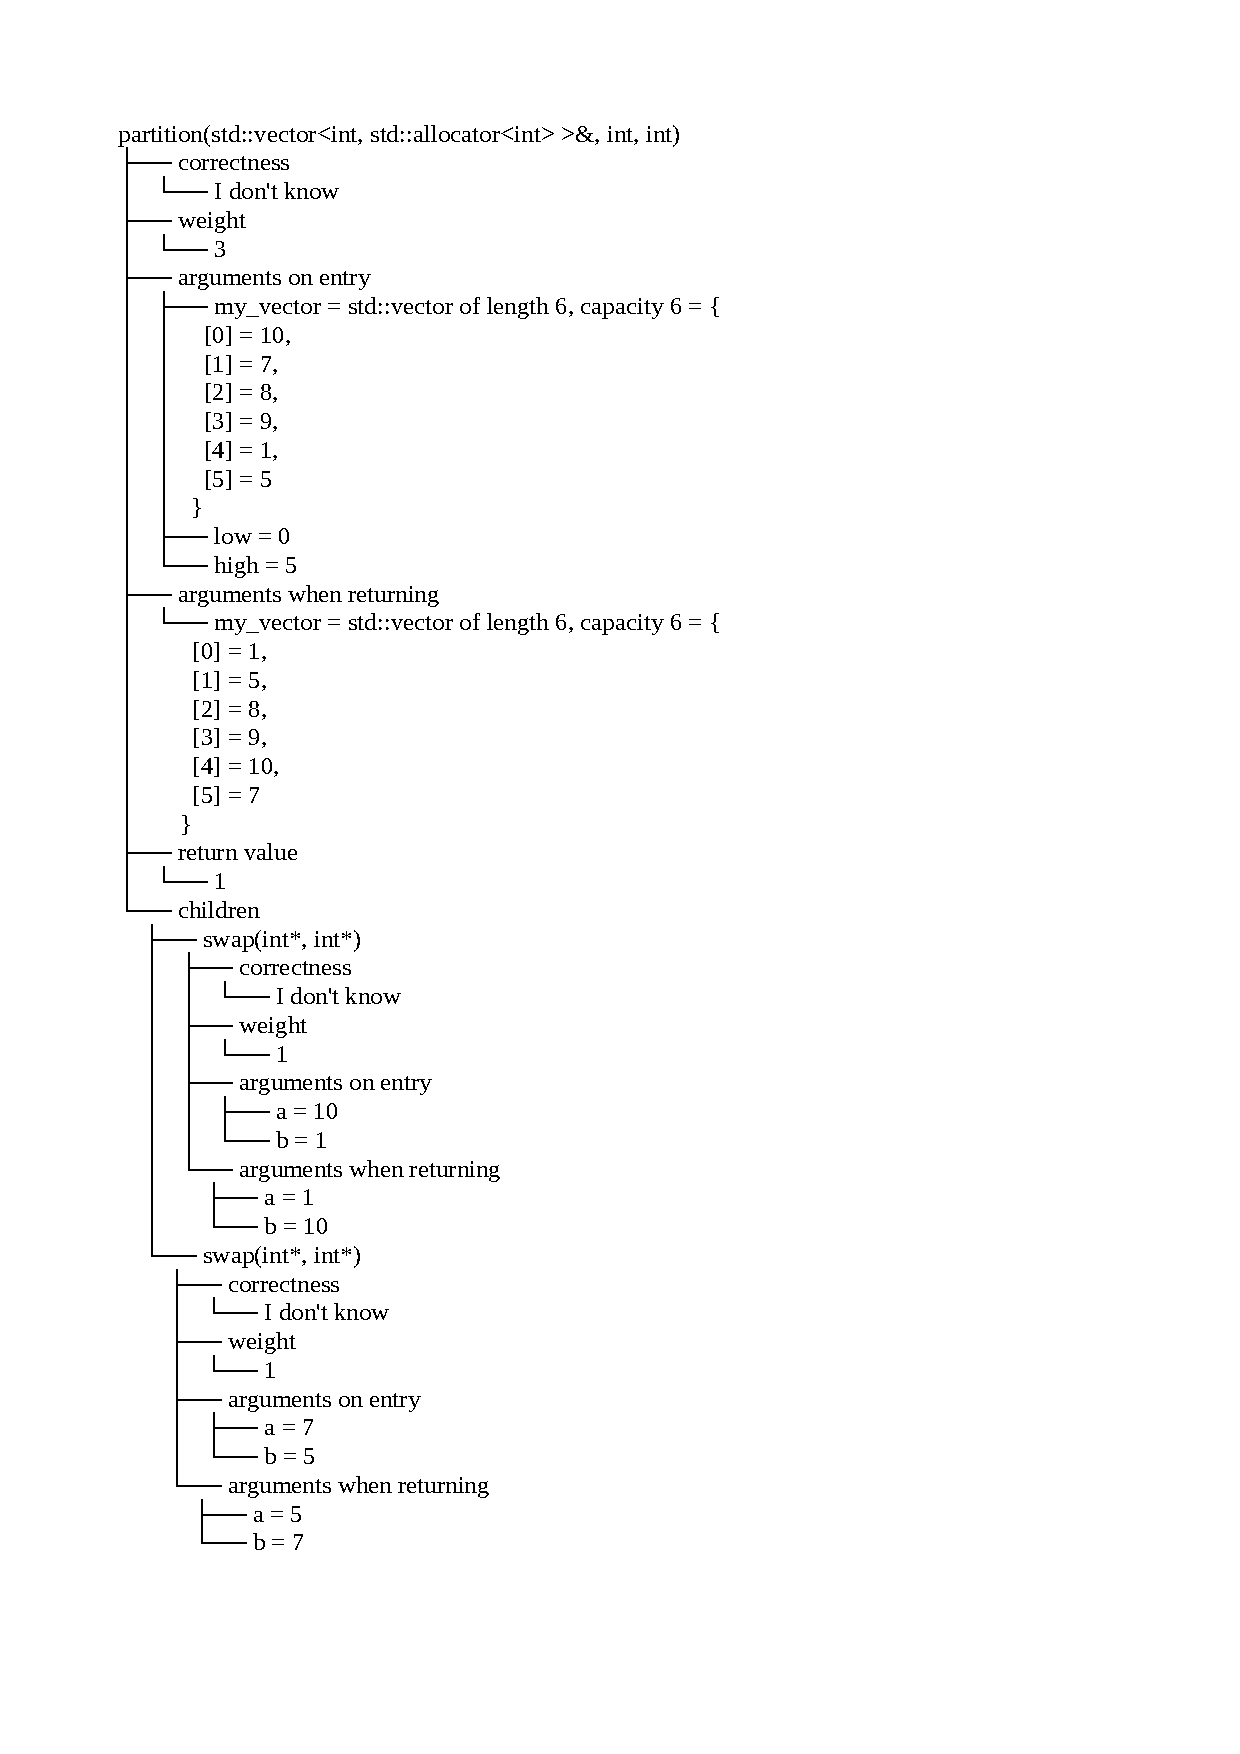
\includegraphics[width=\textwidth,height=\textheight,keepaspectratio]{Imagenes/Vectorial/partitionTree.pdf}
\end{figure}

\begin{definition}[Intended interpretation]
The intended interpretation of a function or method \(f\) given an input set \(I\), denoted \(\mathit{II}_f(I) \to O'\), is a mapping from \(I\) to \(O'\), where \(O'\) is the expected result of executing \(f(I)\).
\end{definition}
\begin{definition}[Wrong node]
A wrong node \(n_{wrong} = f(I) \to O\) is a node that is not equal to its intended interpretation, \(\mathit{II}_f(I) \to O'\).
\end{definition}
\begin{definition}[Correct node]
A correct node is a node that is equal to its intended interpretation.
\end{definition}
\begin{definition}[Buggy node]
A buggy node is a wrong node in which all its children are correct nodes. 
\end{definition}
\theoremstyle{definition}
\begin{exmp}
Figure~\ref{fig:intendedInterpretationSwap} is the intended interpretation of swap \(\mathit{II}_{swap}(I) \to O'\), \(I\) being two pointers pointing to 10 and 1, respectively.
On the other hand, Figure~\ref{fig:buggySwap} is the node \(n_{swap}(I) \to O\) of the execution of swap given the same arguments.
Since \(O'\neq O\) (note that in Figure \ref{fig:buggySwap} swap returns \(a = 10\) and \(b = 1\), whereas in Figure~\ref{fig:intendedInterpretationSwap} \texttt{swap} returns \(a = 1\) and \(b = 10\)), we can say that \(n_{swap}\) is a buggy node, and therefore there is a bug in the function \(swap\), as we will see later.

\begin{figure}[h]
\caption{Intended interpretation of swap function given pointer a to 10 and pointer b to 1}
\label{fig:intendedInterpretationSwap}
\begin{verbatim}
swap(int*, int*)
├── arguments on entry
│   ├── a = 10
│   └── b = 1
└── arguments when returning
    ├── a = 1
    └── b = 10
\end{verbatim}
\end{figure}

\begin{figure}[h]
\caption{Buggy node representing the execution of swap}
\label{fig:buggySwap}
\begin{verbatim}
swap(int*, int*)
├── correctness
│   └── no
├── weight
│   └── 1
├── arguments on entry
│   ├── a = 10
│   └── b = 1
└── arguments when returning
    ├── a = 10
    └── b = 1
\end{verbatim}
\end{figure}

\end{exmp}

\begin{definition}[Detected errors]
When our debugger returns a buggy node \(n_{buggy} = f(I) \to O\), an error in the definition of \(f\) has been detected. 

\end{definition}
\begin{definition}[Navigation strategy]
A navigation strategy is a traversal of the WMDT in which the debugger asks an oracle to answer questions about the correctness of certain nodes, the possible answers being correct or wrong.  
\end{definition}
\begin{definition}[Top-down strategy]
The top-down strategy is a navigation strategy in which when a node is deemed wrong, one of its children is asked; if it is deemed
correct, one of its siblings is asked \cite{surveyStrategies}.
%3.0.2. Top-Down Search (Av-Ron, 1984)
%http://personales.upv.es/josilga/papers/SurveyADS.pdf
\end{definition}
\newtheorem{theorem}{Theorem}
\begin{theorem}[Completeness]
%Completion theorem
Let \(T = (N,E,W,M)\) be a weighted marked debugging tree, \(S\) the top-down strategy, and the root node of \(T\) a wrong node.
If \(S\) receives T as input, it always terminates, producing a node \(n'\in N\) as output.
\end{theorem}
\begin{proof}
See \cite{DeclarativeErrorDiagnosis}.
\end{proof}
\begin{theorem}[Soundness]
%Soundness theorem
Let:
\begin{itemize}
    \item \(T = (N,E,W,M)\) be a weighted marked debugging tree,
    \item the root of T a wrong node,
    \item F a total function such that for every node \(n\in N\) there is a function or method \(f\) such that \(F:n\to f\),
    \item \(\mathit{II}\) a total function such that for every function or method \(f\in F\) there is an intended interpretation \(\mathit{II}_f\) such that \(\mathit{II}:f\to \mathit{II}_f\),
    \item G a total function such that for every node \(n\in N\) there is 3-tuple of inputs \(I\) such that \(G:n\to I\), and
    \item S the top down strategy.
\end{itemize}

If \(S\) receives \(T\) as input, then:
\begin{itemize}
    \item \(S\) returns a node \(n'\),
    \item \(n'\in N\),
    \item \(F(n') = f'\),
    \item \(\mathit{II}(f') = II_{f'}\),
    \item \(G(n') = I\), and
    \item \(\mathit{II}_{f'}(I)\neq f'(I)\).
\end{itemize}
\end{theorem}
\begin{proof}
See \cite{DeclarativeErrorDiagnosis}.
\end{proof}

